\section{Additional material on Section~\ref{sec:trending}}\label{sec:appendix-trending}

\subsection{Data generation for Section~\ref{sec:trending}}\label{subsec:app-trending-data-generation}

The first dataset is generated by sequentially generating $\diffx$ and $\diffy$.
First, the $\diffxt$ are sampled as a sum of a standard normal random number and a uniform random number on $(-10, 10)$:
\begin{equation*}
    \diffxt \sim N(0, 1) + U(-10, 10) \quad t = 1, \dots, T.
\end{equation*}
Subsequently, the $\diffy$ are simulated for a constant trending ratio $k$ by
\begin{equation*}
    \diffyt = \diffxt \cdot n_t * b_t,
\end{equation*}
where $n_t$ is a truncated normal distribution with mean 1 and standard deviation 0.5, truncated at 0 and a symmetric Bernoulli random variable with parameter $k$.
For a time-varying trending ratio, the parameter $k$ is modified to have a wave-shape over time, that is,
\begin{equation*}
    k_t = 0.75 + \sin(t / 365.25 \cdot 2 \pi) / 4,
\end{equation*}
where $T^\star$ is $T$ divided by the number of oscillations; in this case, 4.
For the asymmetric trending ratio, $k$ is a function of $\diffxt$,
\begin{equation*}
    k(x) = 0.5 + \min \left\{ \max \left\{ \frac{x + 5}{10}, 0  \right\} , 1 \right\} / 2.
\end{equation*}

In the second approach, $\diffyt$ and $\diffxt$ are modelled to be multivariate normal with mean 0 and covariance matrix
\begin{equation*}
    \Sigma = \begin{pmatrix} 4 & 3 \\ 3 & 4 \end{pmatrix}.
\end{equation*}
Thus, the conditional probability of trending can be calculated by a conditional normal distribution to
\begin{equation*}
    P(\diffyrv \diffxrv > 0 | \diffxrv = x) = \Phi \left( \frac{3}{4 \sqrt{7}} x \right),
\end{equation*}
where $\Phi$ is a standard normal \ac{cdf}.

The four-quadrant plots for the sample realizations of the data generation schemes are shown in Figure~\ref{fig:appendix_dgps}.

\begin{figure}
    \centering
    \begin{subfigure}{0.24\textwidth}
        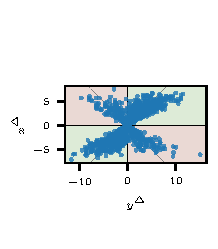
\includegraphics{plots/illustrative_examples/appendix_4q_dgp1}
        \caption{Constant trending ratio.}
    \end{subfigure}\hspace{0.01\textwidth}
    \begin{subfigure}{0.24\textwidth}
        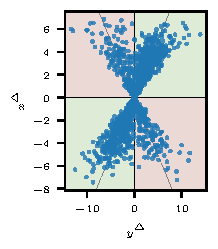
\includegraphics{plots/illustrative_examples/appendix_4q_dgp1_time}
        \caption{Time-varying trending ratio}
    \end{subfigure}\hspace{0.01\textwidth}
    \begin{subfigure}{0.24\textwidth}
        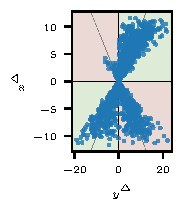
\includegraphics{plots/illustrative_examples/appendix_4q_dgp1_asym}
        \caption{Asymmetric trending ratio}
    \end{subfigure}\hspace{0.01\textwidth}
    \begin{subfigure}{0.24\textwidth}
        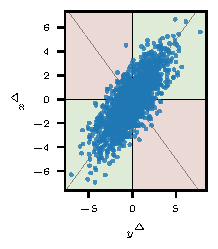
\includegraphics{plots/illustrative_examples/appendix_4q_dgp2}
        \caption{Second approach}
    \end{subfigure}
    \caption{Four-quadrant plots for sample realizations of the data generation schemes of Section~\ref{subsec:app-trending-data-generation}. Although the first and second plot differ over time, their difference is not discernible in the plots. The third data set's asymmetry is visible in the plot but the decrese of trending ability near 0 is not visible. }
    \label{fig:appendix_dgps}
\end{figure}

\subsection{Simulation study on bootstrapping confidence intervals}\label{subsec:app-trending-bootstrap}
We vary the number of available time steps $T$ to be a typical time-series value, such as 30 for daily data in a month, 52 for weekly data, 168, 365, 720, and 1024.
The considered datasets are outlined in Appendix~\ref{subsec:app-trending-data-generation}, the first dataset with asymmetric dependence.
In the calculations, the \verb|scipy| package's implementation of bootstrap confidence intervals is used~\parencite{Virtanen2020}.
The prescribed confidence level is 90 \%, and the number of bootstrap samples is $10,000$.
The share of confidence intervals covering the true values per method and $T$ are shown in Table~\ref{tab:trending_bootstrap}.
The true values of the accuracy are computed based on a dataset of size $10^8$, yielding 0.7501 and 0.7700 for the two datasets.
The computation times per method and dataset are shown in Figure~\ref{fig:trending_bootstrap_time}.
For the small sample sizes up to $T = 168$, only the \ac{bca} method keeps the confidence interval size and yields slightly wider confidence intervals.
The method's results do not differ for the larger sample sizes.
The computation time for the \ac{bca} method is slightly larger than for the other methods, but all methods have a moderate computation time.

\begin{table}
    \centering
    \begin{subtable}{.48\textwidth}
        \begin{tabular}{llll}
\toprule
 & percentile & basic & bca \\
\midrule
30 & 0.84 (0.249) & 0.86 (0.250) & 0.91 (nan) \\
52 & 0.89 (0.194) & 0.89 (0.193) & 0.89 (0.198) \\
168 & 0.91 (0.109) & 0.90 (0.109) & 0.90 (0.110) \\
365 & 0.90 (0.074) & 0.90 (0.074) & 0.90 (0.074) \\
720 & 0.90 (0.053) & 0.90 (0.053) & 0.90 (0.053) \\
1024 & 0.90 (0.044) & 0.90 (0.044) & 0.89 (0.044) \\
\bottomrule
\end{tabular}

        \caption{First dataset}
    \end{subtable}\hspace{0.02\textwidth}
    \begin{subtable}{.48\textwidth}
        \begin{tabular}{llll}
\toprule
 & percentile & basic & BCa \\
\midrule
30 & 0.87 (0.243) & 0.88 (0.242) & 0.92 (0.249) \\
52 & 0.87 (0.188) & 0.89 (0.188) & 0.90 (0.192) \\
168 & 0.89 (0.106) & 0.90 (0.106) & 0.90 (0.107) \\
365 & 0.90 (0.072) & 0.90 (0.072) & 0.90 (0.072) \\
720 & 0.90 (0.052) & 0.90 (0.052) & 0.90 (0.052) \\
1024 & 0.89 (0.043) & 0.90 (0.043) & 0.90 (0.043) \\
\bottomrule
\end{tabular}

        \caption{Second dataset}
    \end{subtable}
    \caption{Proportion of bootstrapping confidence intervals covering the true value of trending ratio per method and sample size $T$. The average width of the confidence interval is listed in brackets.}
    \label{tab:trending_bootstrap}
\end{table}

\begin{figure}
    \centering
    \begin{subfigure}{0.48\textwidth}
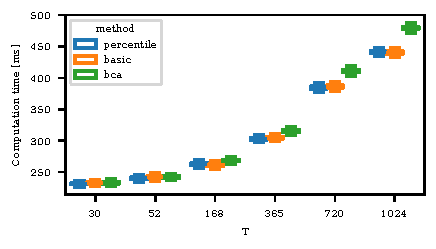
\includegraphics{plots/illustrative_examples/boxplot_comp_time_butterfly}
        \caption{First dataset}
    \end{subfigure}
    \begin{subfigure}{0.48\textwidth}
    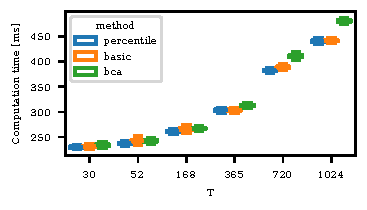
\includegraphics{plots/illustrative_examples/boxplot_comp_time_normal}
        \caption{Second dataset}
    \end{subfigure}
    \caption{Boxplot of the computation time of the different bootstrapping method and data set sizes $T$. The computation time refers to bootstrapping one confidence interval based upon $10,000$ values. Each boxplot reflects $10,000$ samples. The \ac{bca} method takes slightly longer than the other two, but the difference is negligible.}
    \label{fig:trending_bootstrap_time}
\end{figure}

